%\title{Overleaf Memo Template}
% Using the texMemo package by Rob Oakes
\documentclass[letter,12pt]{texMemo}
\usepackage[english]{babel}
\usepackage{color, listings, graphicx, float, booktabs, multirow, outlines}
\pagenumbering{gobble}

%% Edit the header section here. To include your
%% own logo, upload a file via the files menu.
%\memoto{}
\memofrom{Kyle Salitrik | UserID: kps168 | PSU ID: 997543474}
\memosubject{SQL Queries for Generating Schedules}
\memodate{October 19, 2017}
%\logo{
\includegraphics[width=0.3\textwidth]{Overleaf-logo.jpg}}
\graphicspath{{./figures/}}

\definecolor{codegreen}{rgb}{0,0.6,0}
\definecolor{codegray}{rgb}{0.5,0.5,0.5}
\definecolor{codepurple}{rgb}{0.58,0,0.82}
\definecolor{backcolour}{rgb}{0.97,0.97,0.97}
 
\lstdefinestyle{mystyle}{
    %backgroundcolor=\color{backcolour},   
    basicstyle=\footnotesize,
    breakatwhitespace=false,         
    breaklines=true,                 
    captionpos=b,                    
    keepspaces=true,                 
%    numbers=left,                    
%    numbersep=5pt,                  
    showspaces=false,                
    showstringspaces=false,
    showtabs=false,                  
    tabsize=2
}
 
\lstset{style=mystyle}


\begin{document}
\maketitle

\section*{Code Used for Queries}
This following code block shows the SQL queries used to generate the data.
\lstinputlisting[language=SQL]{./code/queries.sql}

\section*{Query Results}
\subsection*{Query 1}
\lstinputlisting[language=SQL]{./code/query1.txt}

\subsection*{Query 2}
\lstinputlisting[language=SQL]{./code/query2.txt}

\subsection*{Query 3}
\lstinputlisting[language=SQL]{./code/query3.txt}

\subsection*{Query 4}
\lstinputlisting[language=SQL]{./code/query4.txt}

\subsection*{Query 5}
\lstinputlisting[language=SQL]{./code/query5.txt}

% \subsection*{Query 6}
% \lstinputlisting[language=SQL]{./code/query6.txt}


%\bigskip{}\decorativeline\bigskip{}
%
%Sincerely,\\
%
%\quad Kyle Salitrik

\newpage
\begin{figure}[H]
	\centering
	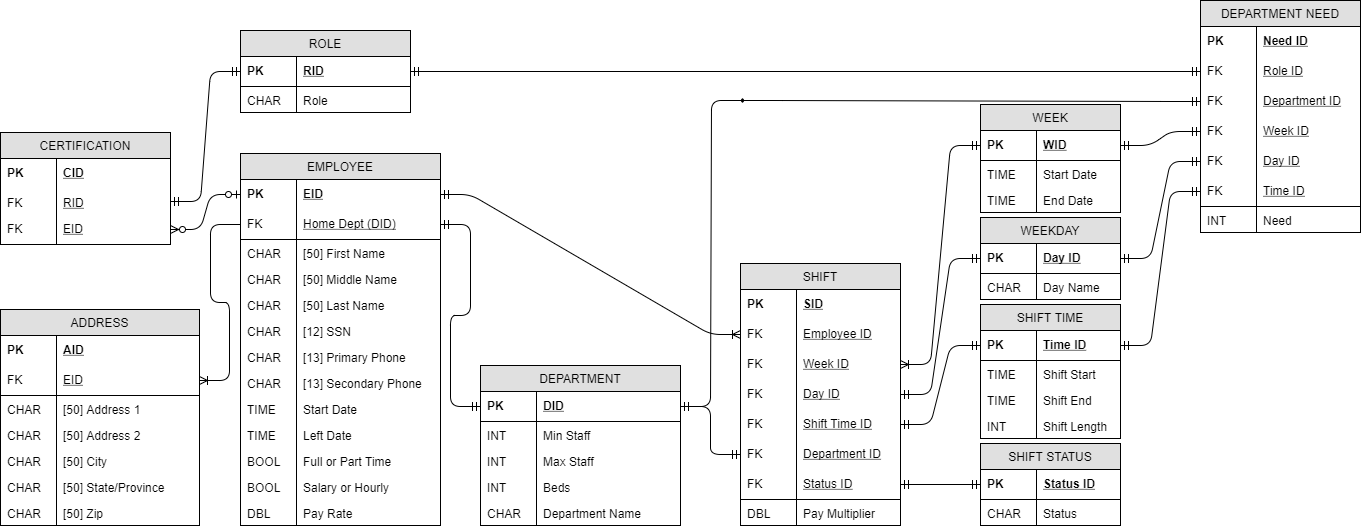
\includegraphics[angle=90, height=\textheight]{er_diag.png}
\end{figure}

\end{document}